\section{Introduction and System Overview}
\label{sec:Intro}

Configuration errors are one of the most important root-causes of
modern software system failures~\cite{xu15systems,yin11anempirical}.
In practice, misconfiguration problems may result in security
vulnerabilities, application crashes, severe disruptions in software
functionality, and incorrect program executions%
~\cite{xu15systems,zhang14encore,yuan11context}.  Although several
tools have been proposed to automate configuration error diagnosis
after failures occur~\cite{wang04automatic,attariyan10automating,
su07autobash,whitaker04configuration}, these tools rely on a manual approach
  to understand and detect the failure symptoms. The main reasons for this are:
  1) entries in configuration files are untyped assignments, 2) there
  is no explicit structure policy for the entries in configuration
  files, and 3) there are surprisingly few rules specifying the
  entries' constraints.

We propose an approach to the verification of  
configuration files which is based on learning rules about the language 
model for configuration files. 

\begin{figure}[t] \centering
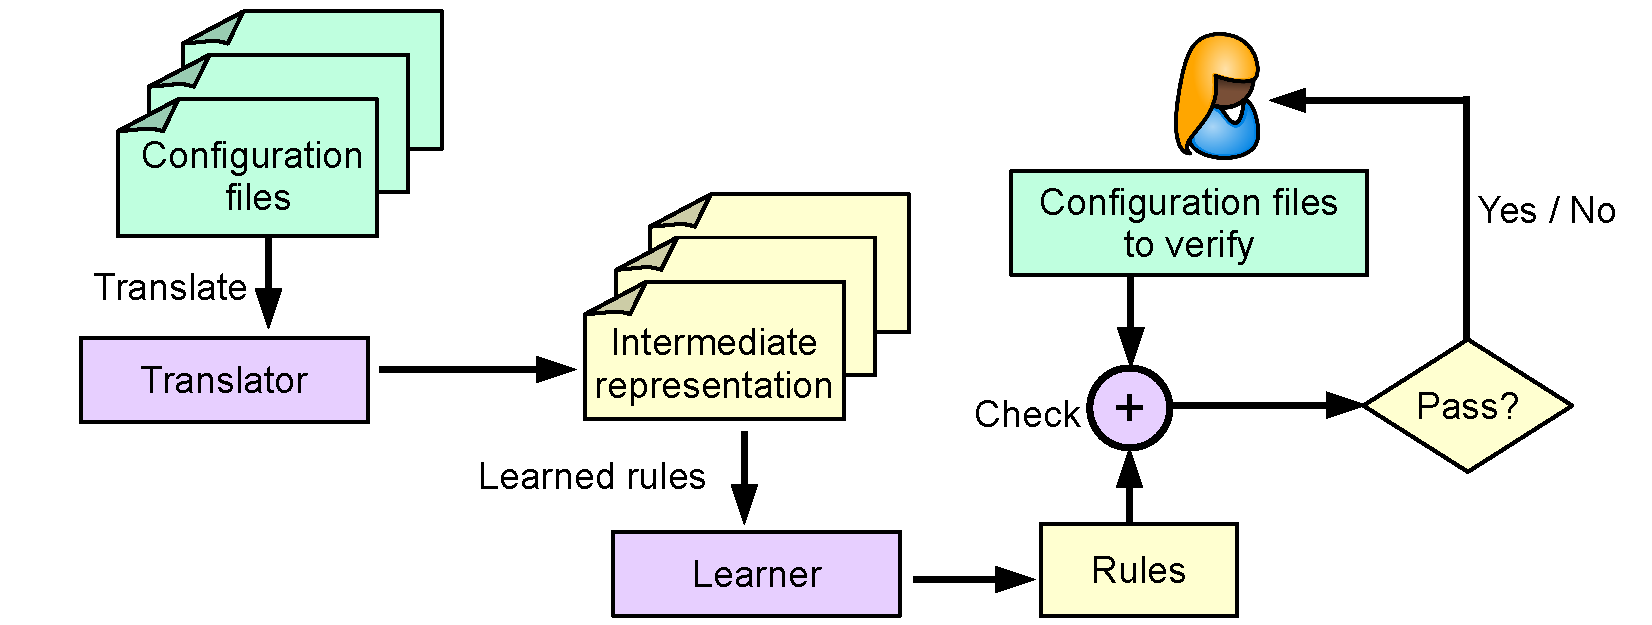
\includegraphics[width=0.63\textwidth]{figs/overview}
\caption{{\footnotesize \app's workflow. The green boxes represent configuration files,
  including both correct general configuration files and users' input
  configuration files. The purple boxes are the components within \app.
  The yellow boxes are results generated by \app's components.}}
\label{fig-overview}
\end{figure}

Figure~\ref{fig-overview} describes an overview of our system. We start
with the assumption that we are given a number of correct configuration
files belonging to the same category (for instance, MySQL or
Apache). Such files follow similar patterns, which we exploit
in a learning algorithm to build rules that
describe a language model for the files. Since the
``language'' of configuration types is untyped and unstructured, we
first parse the files and translate them into a more structured,
intermediary representation.
When running type inference on a configuration file, the type of a variable cannot always be fully determined from a single value.
We address this problem by introducing so called {\emph{probabalistic types}}.
Rather than giving a variable a single type, we assign several types with their probability distributions. 
We can then use these more structured files
as a training set to learn the rules. The learning algorithm
is template-based to be easily extensible. We provide an initial set of templates and the
learner learns some concrete instances from the training set. These
rules are used for detecting errors violating the learned constraints
in the files given by the user.

As an 
illustration of a simple rule that we can learn, consider a template
 $X_1 \le X_2$, where $X_1$ and $X_2$ are
integer variables. The learner might derive the rule stating that
$\texttt{mysql.max\_persistent} \le \texttt{max\_connections}$. There is a classification and taxonomy of configuration errors in the 
existing work on automated configuration troubleshooting~\cite{yin11anempirical, configdataset}. We provide templates for every class that \app can handle: we consider integer constraints, ordering
constraints, typing constraints, and constraints about correlated entries (such as ``if $X$ is present, $Y$ has to appear as well''). 
Unfortunately, we cannot handle the class of errors that rely on the analysis of the whole operating system.
Our language-based approach can only learn on sets of text files, not the system environment.

From a practical perspective \app introduces no additional burden 
to the users: they can simply use \app to check for errors in their configuration files. However, they can also easily extend the framework themselves. The system is designed to be highly modular. If there is a class of rules that \app is not currently learning, the user can develop their own templates and learners for that class. The new learner can be added to \app and this way it can check additionally a new set of errors.

Finally, from a systems perspective this is the first approach that {\emph{proactively}} checks 
 the correctness of configuration files. All previous work
~\cite{xu15systems,zhang14encore,yuan11context, wang04automatic,attariyan10automating,
su07autobash,whitaker04configuration} tries to identify the problem after the
failure occured. Our approach isolates potential errors before the system failure occurs, e.g. before the installation. We can also see \app as a tool that can run in conjunction with existing tools. Pre-analyzed configuration files are already free from language-based errors, and this way the workloads of post-failure forensics at the runtime
is significantly reduced, thus making these tools truly practical.

To summarize, this tool papers makes the following contributions:

\begin{enumerate}

  \item We designed and implemented a tool, \app, that can learn a
language model from an example set of correct configuration files, and
we use the model to verify new configuration files.
  \item We use probabilistic types to assign a confidence distribution over a set of types to a value.
  \item In \app we define a interface for describing a verification attribute in a learning context, making it easy to add new rules to the system.

\end{enumerate}
